% =====================================================================
%  Final Exam Poster  |  A1 landscape  |  tikzposter
%  Output name: Kurmangazykyzy_Karimova_FinalPoster.pdf
%  Overleaf: Menu -> Compiler = pdfLaTeX. Upload every file of this folder.
% =====================================================================
\documentclass[17pt, a1paper, landscape, margin=0mm, innermargin=14mm,
               blockverticalspace=8mm, colspace=12mm, subcolspace=0mm]{tikzposter}

\usepackage[T1]{fontenc}
\usepackage[scaled=0.95]{helvet}          % one font family (Helvetica)
\renewcommand{\familydefault}{\sfdefault}
\usepackage{sfmath}
\usepackage{graphicx, amsmath, booktabs, tabularx, array, multicol, colortbl}
\usepackage{cite}
\usetikzlibrary{positioning}
\usepackage{caption}
\captionsetup{font={normalsize}, labelfont={bf}, labelsep=period, skip=6pt,
              justification=centering}
\captionsetup[figure]{name=Figure}
\usepackage{enumitem}
\setlist[itemize]{leftmargin=1.1em, itemsep=5pt, topsep=4pt, parsep=0pt}

% ---------------- colours: purple, lavender, warm grey ----------------
\definecolor{plum}{HTML}{4B2A7B}       % title bar, headings
\definecolor{violet}{HTML}{6E4BA8}     % accents
\definecolor{lavender}{HTML}{F1ECF8}   % soft boxes
\definecolor{frame}{HTML}{3A3A3A}      % thin section frames
\definecolor{ink}{HTML}{222222}

\definecolorstyle{SoftPurple}{
  \colorlet{colorOne}{plum}\colorlet{colorTwo}{violet}\colorlet{colorThree}{lavender}
}{
  \colorlet{backgroundcolor}{white}
  \colorlet{framecolor}{frame}
  \colorlet{titlefgcolor}{white}
  \colorlet{titlebgcolor}{plum}
  \colorlet{blocktitlebgcolor}{white}
  \colorlet{blocktitlefgcolor}{plum}
  \colorlet{blockbodybgcolor}{white}
  \colorlet{blockbodyfgcolor}{ink}
  \colorlet{innerblocktitlebgcolor}{white}
  \colorlet{innerblocktitlefgcolor}{ink}
  \colorlet{innerblockbodybgcolor}{white}
  \colorlet{innerblockbodyfgcolor}{ink}
  \colorlet{notefgcolor}{ink}\colorlet{notebgcolor}{white}\colorlet{noteframecolor}{frame}
}
\usecolorstyle{SoftPurple}
\usebackgroundstyle{Empty}
\tikzposterlatexaffectionproofoff

% Title: full-width plum bar
\definetitlestyle{PlumBar}{
  width=\paperwidth, roundedcorners=0, linewidth=0pt, innersep=9mm,
  titletotopverticalspace=0mm, titlegraphictotitledistance=0mm
}{
  \fill[plum] (\titleposleft,\titleposbottom) rectangle (\titleposright,\titlepostop);
}
\usetitlestyle{PlumBar}
\makeatletter
\gdef\TP@maketitle{%
  \centering\color{white}
  {\bfseries\fontsize{44}{52}\selectfont\@title\par}
  \vspace{7mm}
  {\fontsize{28}{34}\selectfont\@author\par}
  \vspace{3mm}
  {\fontsize{23}{28}\selectfont\@institute\par}
}
\makeatother

% Blocks: thin dark frame so sections stay apart, heading underlined in purple
\defineblockstyle{SoftFrame}{
  titlewidthscale=1, bodywidthscale=1, titlecenter,
  titleoffsetx=0pt, titleoffsety=0pt, bodyoffsetx=0pt, bodyoffsety=0pt,
  bodyverticalshift=0pt, roundedcorners=0, linewidth=1.6pt,
  titleinnersep=5mm, bodyinnersep=7mm
}{
  \ifBlockHasTitle
    \draw[draw=frame, line width=1.6pt, fill=white]
      (blockbody.south west) rectangle (blocktitle.north east);
    \draw[violet, line width=2.5pt]
      ([xshift=9mm]blocktitle.south west) -- ([xshift=-9mm]blocktitle.south east);
  \else
    \draw[draw=frame, line width=1.6pt, fill=white]
      (blockbody.south west) rectangle (blockbody.north east);
  \fi
}
\useblockstyle{SoftFrame}

% Soft lavender box (RQs) and plum box (gap, key finding): readable from 2 m
\newcommand{\softbox}[1]{%
  \par\vspace{3mm}\noindent
  \fcolorbox{violet}{lavender}{\parbox{\dimexpr\linewidth-2\fboxsep-2\fboxrule}{\raggedright\vspace{2mm}#1\vspace{2mm}}}\par\vspace{3mm}}
\newcommand{\bigbox}[2]{%
  \par\vspace{4mm}\noindent
  \colorbox{plum}{\parbox{\dimexpr\linewidth-2\fboxsep}{\vspace{4mm}%
    \centering\color{white}{\bfseries\large #1}\par\vspace{2mm}
    {\bfseries\fontsize{25}{31}\selectfont #2\par}\vspace{4mm}}}\par\vspace{4mm}}
\newcommand{\sub}[1]{\par\vspace{5mm}{\color{violet}\bfseries\Large #1}\par\vspace{2mm}}
\makeatletter
\newcommand{\tightlists}{\def\@listi{\leftmargin\leftmargini\topsep0pt\parsep0pt\itemsep1pt}\let\@listI\@listi}
\makeatother
\newcommand{\rqlab}[1]{\textcolor{plum}{\bfseries #1}}

% ---------------------------------------------------------------------
\title{Comparison of Classical and Diffusion-Based Image Inpainting Methods for Photo Restoration: A Pilot Study}
\author{Dilyara Kurmangazykyzy \qquad Saule Karimova}
\institute{Astana IT University \quad\textbullet\quad Group BDA-2405 \quad\textbullet\quad Supervisor: Karashbaeva Zhanat}

\begin{document}
\maketitle[width=\paperwidth, linewidth=0pt, innersep=7mm, titletoblockverticalspace=8mm]

\begin{columns}
% =====================================================================
\column{0.32}
% =====================================================================
\block{Problem and Research Questions}{
Old photographs lose parts of the image to scratches, tears and stains, and restoring them by hand is slow \cite{kuo2022}. Image inpainting fills the missing parts from the remaining pixels with classical or diffusion-based methods \cite{kuo2022,wang2026}. A method may also add details that were never there, which becomes a factual error in photos of real people or events \cite{peng2026dcadif}.
\softbox{%
\rqlab{RQ1.} {\bfseries How do a PDE-based (Navier--Stokes), an exemplar-based (Criminisi) and a diffusion-based (ResShift) method differ in restoration quality at about 5\%, 20\% and 40\% damage?}\par\vspace{3mm}
\rqlab{RQ2.} How much processing time does each method need?\par\vspace{3mm}
\rqlab{RQ3.} Does any method add details that were never in the original photograph?}
}

\block{Literature Synthesis and Research Gap}{
\centering
\captionof{table}{Main inpainting approaches.}
\normalsize
\renewcommand{\arraystretch}{1.25}
\begin{tabularx}{\linewidth}{@{}>{\raggedright\arraybackslash}p{0.27\linewidth}>{\raggedright\arraybackslash}X>{\raggedright\arraybackslash}X@{}}
\rowcolor{lavender}\textbf{Approach} & \textbf{Strength} & \textbf{Limitation}\\
PDE-based \cite{xiao2024} & No training data & Fails on large holes \cite{wang2026}\\
Exemplar-based \cite{xie2022} & Keeps edges & Fails on complex holes \cite{wang2026}\\
Diffusion-based \cite{yue2025} & Coherent structure & Slow, may invent details \cite{peng2026dcadif}\\
\bottomrule
\end{tabularx}
\large\raggedright
\begin{itemize}
  \item Heritage diffusion studies rarely use classical baselines \cite{peng2026dcadif,han2026diffumural}, and the only classical comparison used remote sensing images \cite{sekrecka2025} (Table~1).
  \item Good scores do not rule out invented content \cite{yang2024,han2026diffumural}, and cost is rarely reported next to quality \cite{yue2025}.
\end{itemize}
\bigbox{RESEARCH GAP}{No study has compared classical and diffusion-based methods on damaged photographs and, in the same experiment, measured their time and checked them for invented content.}
}

\block{Methods and Data}{
\centering
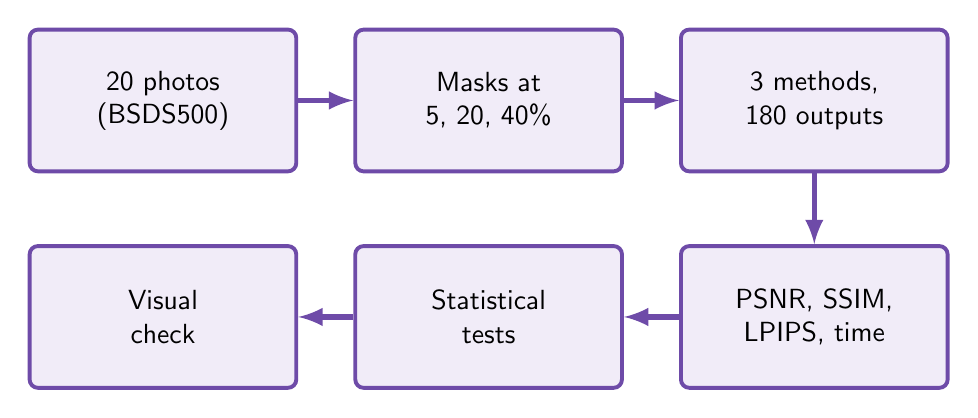
\begin{tikzpicture}[node distance=7mm,
   st/.style={draw=violet, line width=1.4pt, fill=lavender, align=center, minimum height=18mm,
              text width=0.26\linewidth, font=\normalsize, rounded corners=3pt},
   ar/.style={-latex, line width=2pt, violet}]
  \node[st] (a) {20 photos\\(BSDS500)};
  \node[st, right=of a] (b) {Masks at\\5, 20, 40\%};
  \node[st, right=of b] (c) {3 methods,\\180 outputs};
  \node[st, below=9mm of c] (d) {PSNR, SSIM,\\LPIPS, time};
  \node[st, left=of d] (e) {Statistical\\tests};
  \node[st, left=of e] (f) {Visual\\check};
  \draw[ar] (a) -- (b); \draw[ar] (b) -- (c); \draw[ar] (c) -- (d);
  \draw[ar] (d) -- (e); \draw[ar] (e) -- (f);
\end{tikzpicture}
\captionof{figure}{Study workflow.}
\raggedright
\begin{itemize}
  \item \textbf{Data.} 20 BSDS500 test photos \cite{bsds500}, 7 portraits, 7 landscapes and 6 groups, resized to $256\times256$ px.
\end{itemize}
}

% =====================================================================
\column{0.33}
% =====================================================================
\block{}{
\begin{itemize}
  \item \textbf{Damage.} Irregular strokes and blotches imitating scratches, tears and stains, the same mask for every method (Fig.~1).
  \item \textbf{Methods.} Navier--Stokes in OpenCV and our Criminisi code as baselines, pretrained ResShift with 4 steps \cite{yue2025}.
\end{itemize}
\sub{Metrics and analysis \cite{yang2024}}
\vspace{-8mm}
\begin{gather*}
\mathrm{PSNR} = 10\log_{10}\frac{\mathrm{MAX}_I^2}{\mathrm{MSE}}\qquad
\mathrm{SSIM}(x,y) = \frac{(2\mu_x\mu_y + C_1)(2\sigma_{xy} + C_2)}{(\mu_x^2 + \mu_y^2 + C_1)(\sigma_x^2 + \sigma_y^2 + C_2)}\\[2mm]
\mathrm{LPIPS}(x,y) = \sum_l \frac{1}{H_lW_l}\sum_{h,w}\big\lVert\phi_l(x)_{hw}-\phi_l(y)_{hw}\big\rVert_2^2
\end{gather*}
\vspace{-7mm}
\begin{itemize}
  \item Quality and time were compared with Friedman and Holm-corrected Wilcoxon tests \cite{rainio2024}, and invented details by a visual check of the first photo of each type.
\end{itemize}
}

\block{Results}{
\bigbox{KEY FINDING}{The diffusion-based method had the lowest LPIPS in all 20 photos but replaced a face at 40\% damage.}

\sub{Restoration quality}
\centering
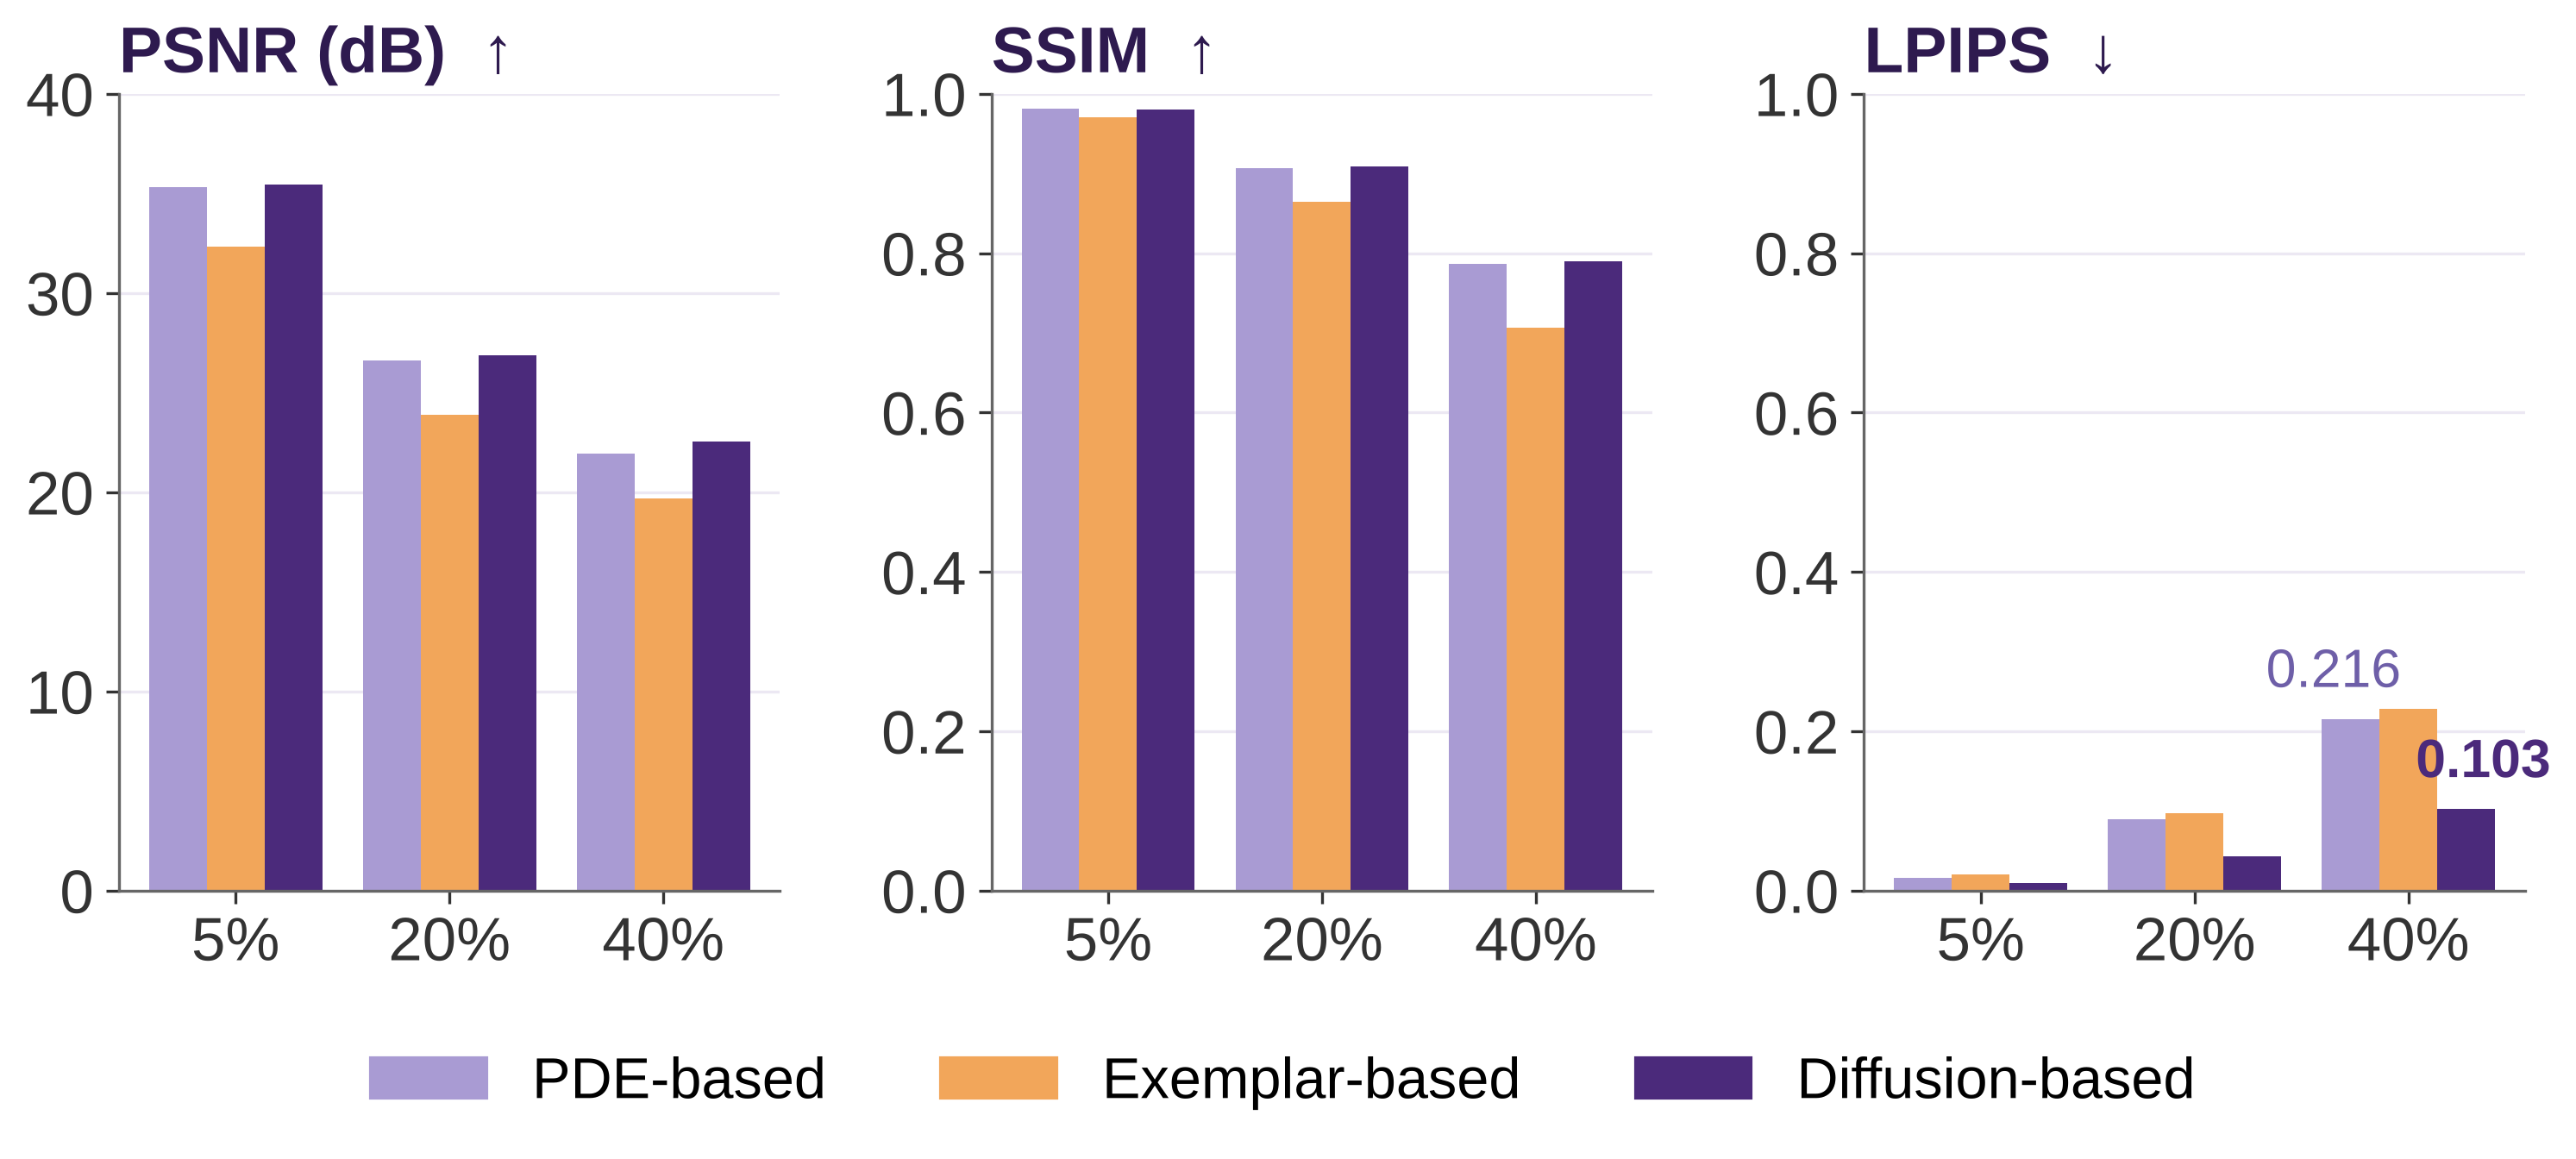
\includegraphics[width=0.84\linewidth]{fig2_quality.png}
\captionof{figure}{Mean quality at each damage level ($n=20$).}
\raggedright
\begin{itemize}
  \item The PDE-based and diffusion-based methods tied on PSNR and SSIM, but at 40\% their LPIPS was \textbf{0.216 and 0.103} (Fig.~2).
  \item The diffusion-based method had the lower LPIPS in \textbf{20 of 20 photos} at every level ($p<.001$). Its PSNR lead was significant only at 40\% ($p=.030$).
\end{itemize}

\sub{Processing time}
\begin{minipage}[c]{0.52\linewidth}
\centering
\captionof{table}{Mean time per image (s).}
\normalsize\renewcommand{\arraystretch}{1.2}
\begin{tabular}{@{}lccc@{}}
\rowcolor{lavender}\textbf{Method} & \textbf{5\%} & \textbf{20\%} & \textbf{40\%}\\
PDE-based & 0.005 & 0.020 & 0.035\\
Exemplar-based & 3.26 & 13.32 & 25.61\\
Diffusion-based & 0.39 & 0.38 & 0.38\\
\bottomrule
\end{tabular}
\end{minipage}\hfill
\begin{minipage}[c]{0.45\linewidth}\raggedright
Only the exemplar-based method slowed down as damage grew, and the order was the same in every photo (Table~2).
\end{minipage}
}

% =====================================================================
\column{0.35}
% =====================================================================
\block{}{
\sub{Invented details}
\centering
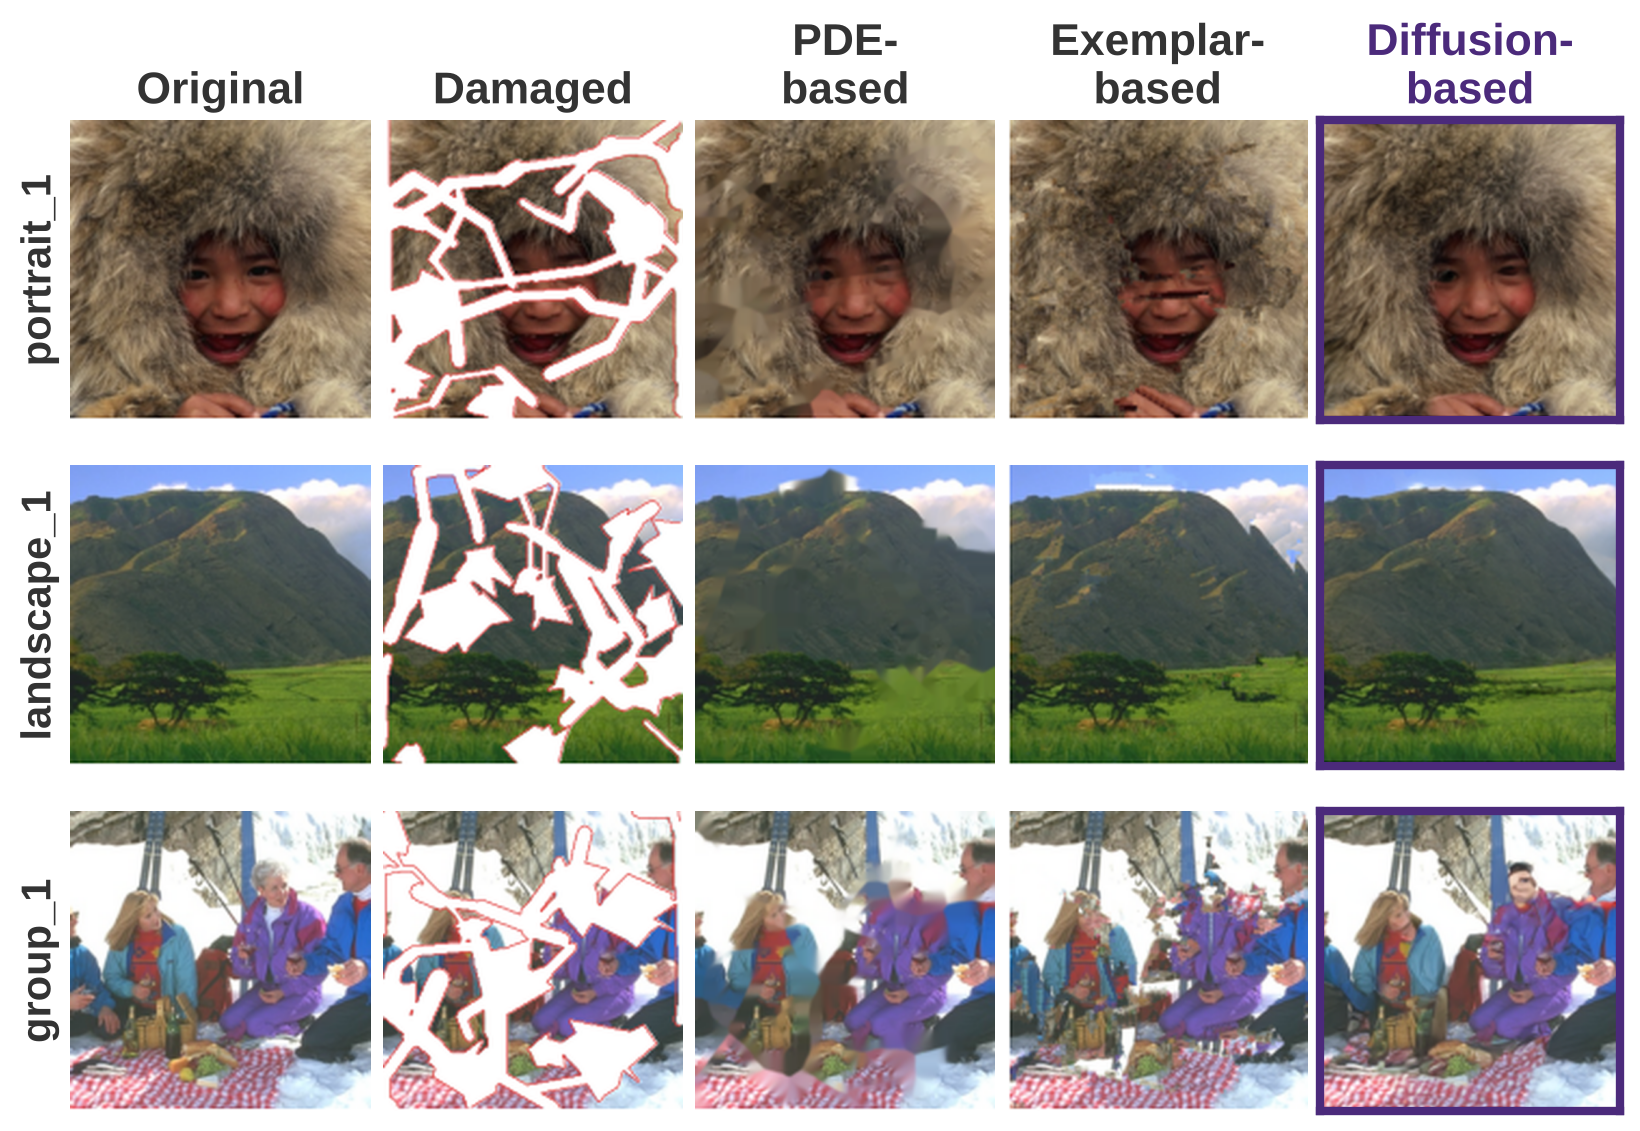
\includegraphics[width=0.72\linewidth]{fig3_visual.png}
\captionof{figure}{Restorations at 40\% damage. Photos from BSDS500 \cite{bsds500}.}
\raggedright
\begin{itemize}
  \item The PDE-based method blurred and the exemplar-based method pasted wrong patches (Fig.~3).
  \item The diffusion-based method replaced the white-haired woman in group\_1 with \textbf{a different person}, yet its LPIPS stayed the best.
\end{itemize}
}

\block{Discussion and Conclusion}{
\begin{itemize}
  \item \textbf{Why the scores disagree.} PSNR and SSIM reward a smooth, blurred fill, and LPIPS rewards realistic texture.
  \item \textbf{Why a face changed.} A generative model paints what is likely, not what was there.
\end{itemize}
\softbox{%
\rqlab{RQ1.} The diffusion-based method was best on LPIPS and tied with the PDE-based method on PSNR and SSIM.\par\vspace{2mm}
\rqlab{RQ2.} The PDE-based method was fastest and the exemplar-based method slowest.\par\vspace{2mm}
\rqlab{RQ3.} Yes. At 40\% damage a face was replaced, and the scores missed it.}
\textbf{Contribution.} Quality, time and invented content compared in one experiment.\par\vspace{2mm}
\textbf{Recommendation.} Use the diffusion-based method for large damage, with a human check.
}

\block{Limitations and Threats to Validity}{
\begin{itemize}
  \item Simulated damage on 20 small photos, so the tests are exploratory.
  \item One method per family and one seed, so the results hold for ResShift only.
  \item Full-image scores shrink the differences, and only the authors checked visually.
  \item Public dataset with no new photos of people, but invented faces must be disclosed.
\end{itemize}
}
\end{columns}

\block{References}{
\vspace{-7mm}
\footnotesize\tightlists
\renewcommand{\section}[2]{}%  hide the default heading inside the block
\begin{multicols}{4}
\bibliographystyle{IEEEtran}
\bibliography{references}
\end{multicols}
\vspace{-9mm}
}
\end{document}
